%% !TEX TS-program = pdflatexmk
%% !BIB TS-program = bibtex

\documentclass[12pt, a4paper, oneside]{book}
\usepackage{import}
\subimport{../}{preamble}
\ExecuteBibliographyOptions{articletitle=false}
\standalonetrue
\onehalfspacing
\begin{document}

\begin{singlespace}
\color{white}\chapter{Conclusions and Outlook}
\end{singlespace}

\AddToShipoutPictureBG*{ \AtPageUpperLeft{ \put(0,-220)
%{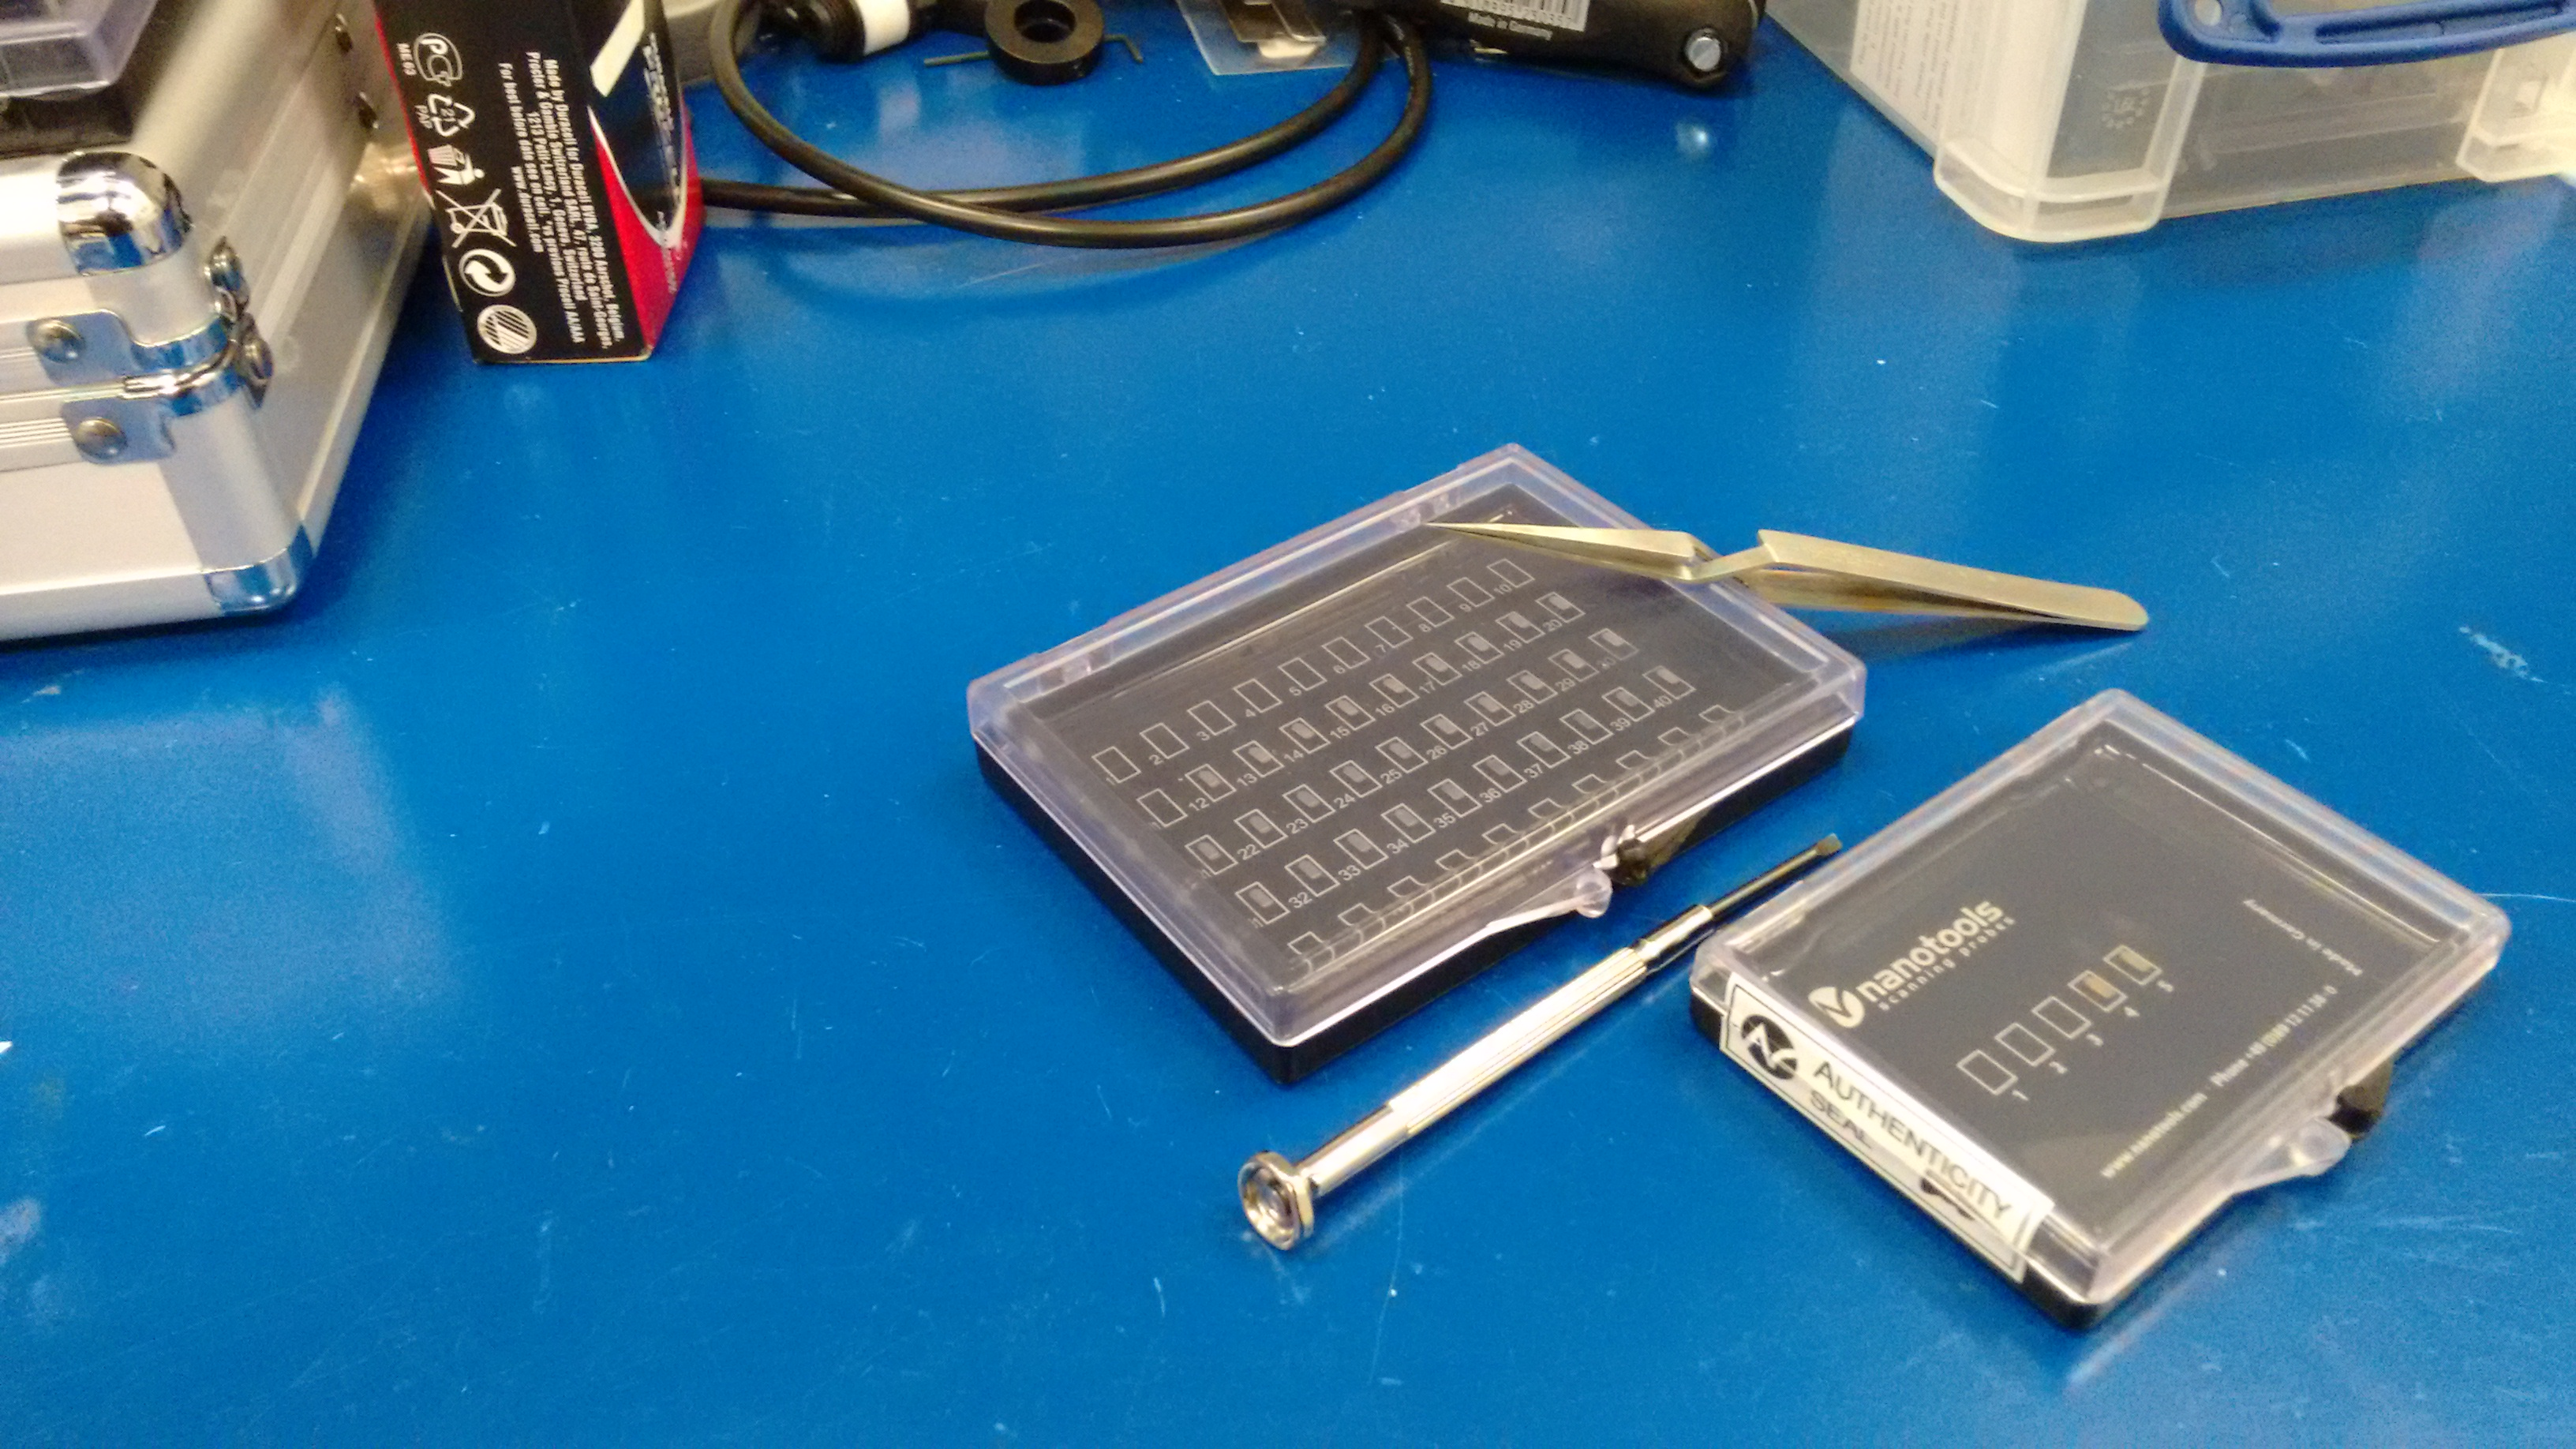
\includegraphics[width=\paperwidth, clip=true, trim=0 80 0 0]{figures/chapter_cover.jpg}}
{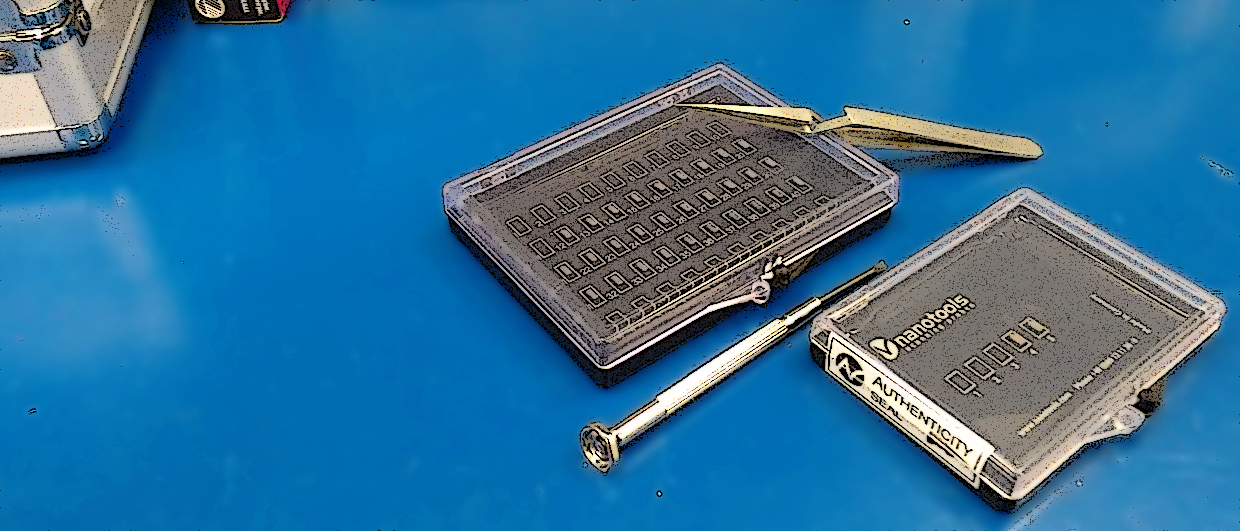
\includegraphics[width=\paperwidth]{../chapter_covers/conclusions_cover.png}}
}}

% Project overview
This project has focussed on the understanding and application of tips for plasmonics, with the aim to use tips to further understand the recently revealed sub-nm regime of plasmonic coupling. Though the initial motivation was to investigate the quantum regime of plasmonic coupling, the project diversified into studying the optical differences between sharp and spherical tips using techniques such as hyperspectral imaging and plasmon coupling, the development of an electrochemical method as an alternative approach to producing spherical tips and the application of plasmonic tips for TERS. Finally, spherical tips were applied to investigate quantum effects in the sub-nm plasmonic coupling regime. Work was therefore split between three core areas: development of plasmonic tips, design and construction of a custom microscope for tip experiments, and ultimately performing experiments on combined tip systems.

% Review of spherical tip fabrication
Failure to observe any plasmonic behaviour in the far-field optical spectra of sharp Au AFM tips, despite their prominence in many near-field enhancing techniques, led to a more in-depth investigation into nanostructured tip geometries. By nanostructuring an AFM tip, some of the well-known antenna-like properties of individual plasmonic nanoparticles are transferred into the AFM probe form factor. The spherical tip geometry, with its radiative plasmons, was selected for simplicity. Both commercially-available spherical Au tips, used in previous tip plasmonics experiments, and AuNP-on-Pt tips, fabricated in-house using a newly developed pulsed electrodeposition procedure, are studied. Pulsed electrodeposition was chosen for its ability to exploit the sharp apex of AFM tips and quickly produce nanostructured tips. The technique was developed from its initial conception through to beginning the optimisation of each parameter in order to improve the process reliability and gain control of the tip morphology. Due to time constraints and the significant effort required to complete other aspects of this project, controllable electrochemical growth of spherically-tipped AFM probes was only partially optimised but produced enough samples to facilitate experiments.
% Work still needed on spherical tip fabrication
Further work is still needed to understand the exact mechanism by which nanoparticles nucleate and grow at and around the apex and optimise each growth parameter. Achieving this would enable a large number of varied studies into the application of plasmonic tips for TENOM - a direction of research only touched upon in current work.

% Review of test rig design chapter
The optical study of AFM tips and the continued probing of dynamic plasmon coupling through each interaction regime necessitated the design of a custom microscope capable of combining the function and stability of two opposing AFM devices with a platform for broadband dark-field spectroscopy. The novel design and robust performance of the microscope has been discussed at length and quantified where appropriate. The comprehensive design of the dual-tip platform meant experiments could implement optical, electronic and force measurements for a more complete characterisation of plasmonic systems than is capable in many other experimental setups. Specifically, the combination of hyperspectral imaging and scanning capacitance microscopy enabled the alignment of AFM tips to each other and to the focus of the incident beam, resulting in a highly reproducible plasmonic dimer arrangement. Additionally, the modular design of the microscope and its array of possible measurements make it adaptable and extensible for many other experiments. Within the scope of this project its main use has been to perform experiments on AFM tips.

% Review of tip plasmonics chapter
Observations of strong optical resonances in spherical Au tips were attributed to radiative localised surface plasmon excitation - a feature not found in sharp metallic tips. The agreement between apex spectra extracted from hyperspectral imaging, broadband tuneable SERS and dynamic plasmon coupling experiments confirm that spherical metallic tips support antenna-like plasmons similar to those in individual nanoparticles, while sharp metallic tips remain unresponsive to light. The spherical Au tip LSP conveniently exists at the commonly used HeNe wavelength leading to enhanced Raman scattering efficiencies, 30$\times$ that of a sharp Au tip. This improvement is a step towards better exploiting controlled nanostructuring of tips for more enhanced and reliable sensing, and promoting radiative approaches to TENOM. However, direct comparison with evanescent excitation methods has not been performed and conclusions remain speculative for the time being.

% Review of quantum tunnelling chapter
The final sets of measurements used pairs of spherical Au tips to target the sub-nm coupling regime. The onset of quantum effects on plasmonic coupling was investigated in ambient conditions, surpassing the earlier experiments performed by Savage et al. \cite{savage2012}. The addition of tunnelling conductance and gap force measurements greatly increased the amount of information extracted from the dimer system to better understand the physics of sub-nm gaps. The robust design of the microscope platform enabled many successful scans through the quantum regime. Measurements showed both the screening of coupled plasmons followed by their transformation into CTPs, correlated with the onset of quantum tunnelling and QPC formation. Observations are in general agreement with the principles underlying recent quantum theoretical descriptions of the quantum regime though further theoretical affirmation of these results is still required. Results strongly suggest the existence of critical conductances which determine the points at which key effects are seen in the quantum regime, a feature which should be further investigated in this and many other systems.

\section{Outlook and Future Directions}

The experiments carried out have both demonstrated the appeal of nanostructured tips and expanded upon the rich regime of quantum plasmonics for further exploration. This project concludes at a pivotal point at which sub-nm gaps can reliably be probed using a newly-developed microscope platform. Within the current experimental system there is still scope for many further projects and many questions still remain regarding the effects of quantum mechanics on plasmonics. Experimental parameters, such as temperature, humidity (gap water content), gap chemical composition (monolayers on tips) and applied bias (non-linear electrical control of coupled plasmons), are currently controllable but investigations into their effects on quantum-scale plasmonic gaps have yet to begin. Other parameters, such as pressure (vacuum), would require some adaptation but investigations remain possible.

Even in its current state the microscope platform could be used to perform a range of new and interesting experiments. Use of an electrical excitation mechanism has yet to be tested but is a realistic aim that could yield interesting results and background-free spectroscopy. Coating tips in both conductive and insulating molecules could be an effective method for determining critical conductances, with direct comparison to recent NPoM systems involving gap spacers \cite{mertens2013, benz2014, cha2014, denijs2014}. Coupling a tip with its mirror charge in an opposing cantilever is also a potential route for dynamically testing plasmonic interactions with molecular spacers. Each of these would provide a new insight into plasmonics on a fundamental level.

Though all results presented within this project focus on large, spherical Au tips, the developed tip fabrication and characterisation techniques are not limited to a specific metal or geometry. It would be interesting to measure and quantitatively compare the scattering response and field enhancement of spherical tips with carefully controlled sphere and neck sizes to validate theoretical predictions, and grow other sphere materials such as Ag, Cu or Al, if such materials electrochemically deposit in a similar manner to Au. A small amount of work was started, with some success, applying pulsed electrodeposition to deposit metal nanostructures other than Au on other conductive AFM tips, such as highly-doped Si. If successful this would facilitate the production of plasmonic probes resonant across a wide range of visible-NIR frequencies.

Finally, more controllable confirmation of quantum effects in plasmonic systems could become possible using \glspl{2deg}, the systems initially used to discover quantised conductivity \cite{van1988quantized, wharam1988one}, and those currently being explored for plasmonics at THz frequencies \cite{koppens2011graphene, christensen2011graphene, chen2012optical}. By gating a biased 2DEG a region can be electrically depleted to form a 1D constriction through which ballistic transport occurs. Thus, by gating a plasmonic 2DEG, it could be controllably depleted to pass through both capacitively coupled and conductive regimes.

To conclude, the recently accessible boundary between the capacitive coupling and charge transfer regimes of plasmonics has been successfully probed and continues to display a wealth of interesting physics. Dynamically controlling the particle positions of an AFM tip dimer has become a powerful experimental technique for the study of such physics. Since smaller gaps, blended with molecular electronics, have begun to become experimentally attainable, the results of these latest experiments are expected to be of great interest to the general plasmonics community. From the point of view of fundamental plasmonics, they provide an insight into a largely unknown regime of plasmonics whilst from an applied aspect they indicate both the limitations of plasmonic sensing and a potential new method for measuring electronic transport at optical frequencies.

\ifstandalone
\begin{singlespace}
\fontsize{8pt}{1em}\selectfont
\printbibliography[notcategory=fullcited]
\end{singlespace}
\fi

\end{document}